\subsection{Tests}
For the testing phase we need to test the extra implementations we made to our vending machine. This led to the creation of our testbench, where we test for 6 different conditions.
\begin{enumerate}
    \item Test of the multiplexor and price of items, along with default value of \texttt{alarm}, \texttt{releaseCan} and \texttt{rejectCoinLED}.
    \item Inserting coins and buying item, test for insufficient funds and buy cheaper item instead.
    \item Holding buy, testing for edge detection.
    \item Testing the cash limit of 99 kroners.
    \item Testing the coin limit of 63 coins.
    \item Testing for empty Vending Machine
\end{enumerate}
These tests all go through and test our extra implementations on our vending machine. Firstly our multiplexor is tested by going through all values. Since the itemPrice is an internal signal it can only be read in the .vcd file. \\
Afterwards we test the buy function, first where we have enough kroners and secondly where we don't have enough, one should pass the other should result in an alarm. Afterwards we do a simple edge detection and hold our buy button for several clock cycles, this should still result in only one attempt to purchase. Lastly we test our hard limits for the vending machine either by inserting a lot of coins and attempting to put more in, than what the capacity allows for.\\
Some things like the blinking of the 4-digit display isn't tested for, given that we did a fully functioning segment display in an earlier lab, and just reused the code from that lab, with the small modification of just changing the \texttt{an} signal (\texttt{activeDigit} in our code), at given situations.\\[1in]

\subsection{Results}
When the Vending Machine has passed all of our test, it is ready to be synthesized down to our FPGA board. Our current design, passes all of the tests. After flashing our FPGA with our design, we did the same edge testing as in our testbench. No errors between the testbench or FPGA were found, the Vending Machine and UART was working as intended. \\
With the whole design finished, we can finally map out the general structure of our Vending Machine. We have a Datapath state(VendingMachine.scala), which communicates with the FSM (VendingFSM.scala) and a third state (UartDisplay.scala) which handles the logic behind which message to send, when given a signal from the Datapath.
The FSMD for our Vending Machine looks like this:
\begin{figure}[H]
    \centering
    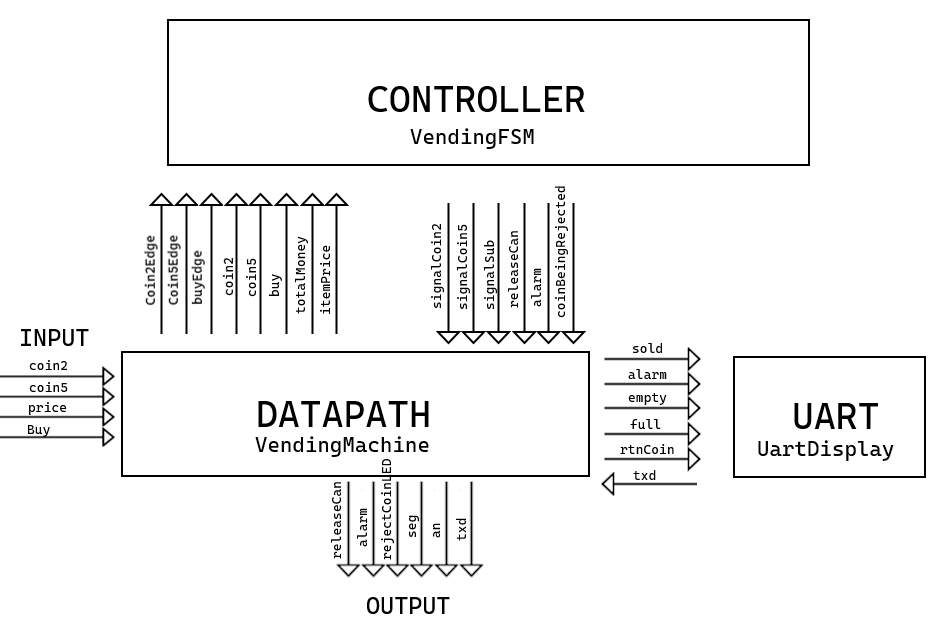
\includegraphics[width=1\linewidth]{root/VendingDatapath.png}
    \label{fig:placeholder}
\end{figure}
When using the vivado synthesizer we can open up the design, and see that our whole circuit is located in the X0Y0 region of the board, We can then see that the design uses 317 LUT's for logic and 166 Registers as FF's.

Along with this we can see that the worst timings for the design is:\\
$t_{setup}=3.398ns$, $t_{hold}=0.193ns$ and $t_{pulse}=4.5ns$ but the total worst delay is a path with $t_{worst}=6.55ns$ of delay. Since our board runs with a speed of 100MHz which translates to a clock of 10ns, all the timings constraint are met. With the critical path in the system being $t_{worst}=6.55ns$ the maximum clock speed for this design is around $\approx153MHz$

This is also the FSM state machine that was produced.
\begin{figure} [H]
    \centering
    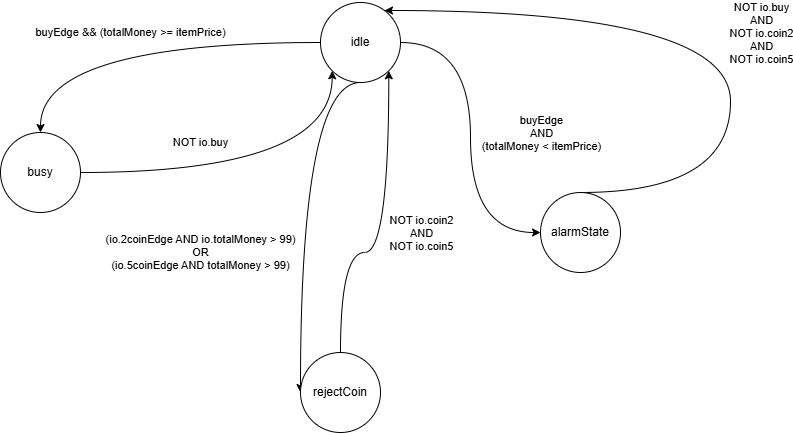
\includegraphics[width=1\linewidth]{root/FSM.png}
\end{figure}
And this is a somewhat simplified sketch of the internal components of the datapath. Some simple logic isn't shown, as that would make the sketch too messy, but this roughly shows the internals of the Datapath.

\begin{figure}[H]
    \centering
    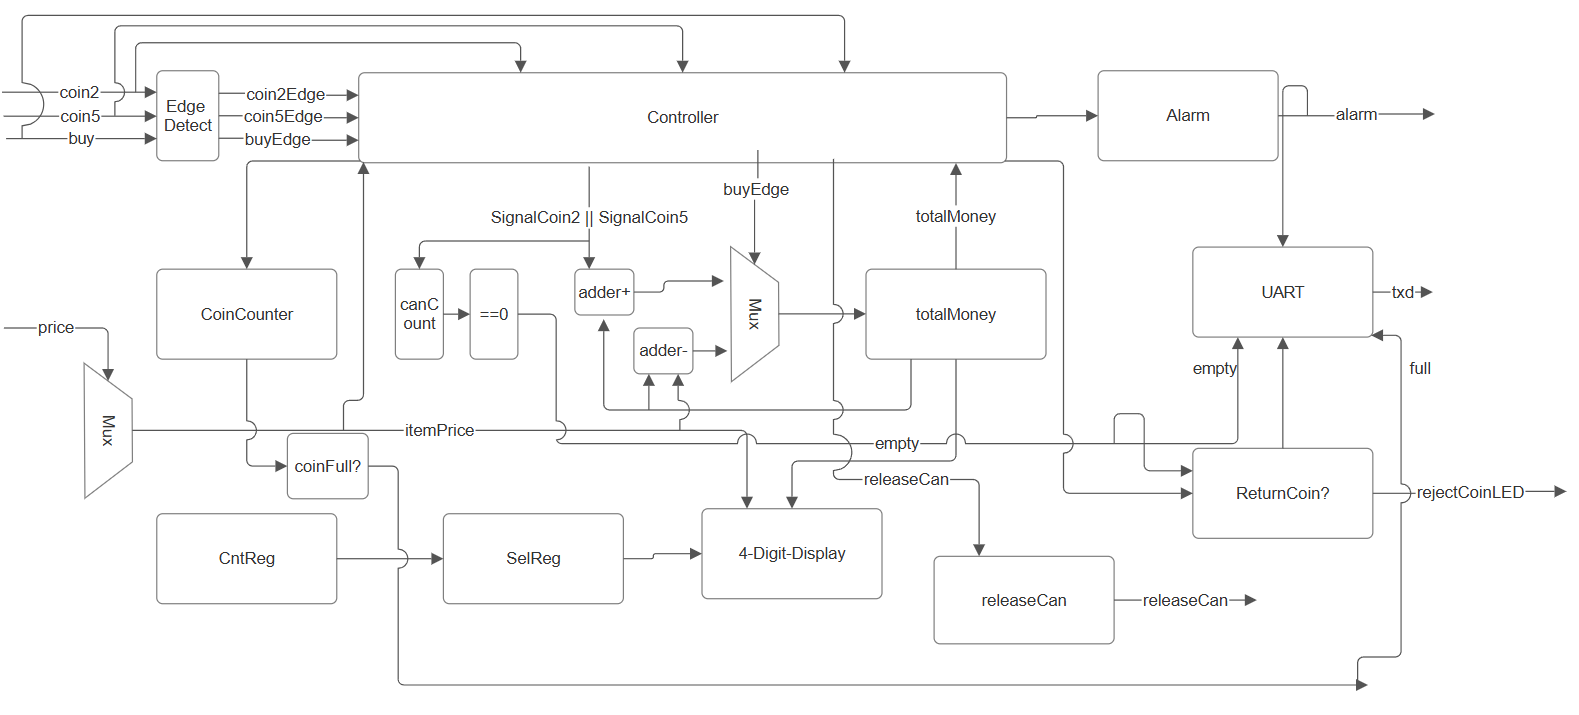
\includegraphics[width=1\linewidth]{root/datapath_internal.png}
    \label{fig:placeholder}
\end{figure}